% !TeX root = ../main.tex
% Add the above to each chapter to make compiling the PDF easier in some editors.

\chapter{Approach}\label{chapter:approach}

In this chapter we introduce the reader to the method for the experiment data collection and analysis for MaCon approach. First we describe the requirements extracted from the problem description and disadvantages of using the existing software solution for usability data logging in the scope of the problem. Then we portray the general approach of fulfilling the requirements and go into more details of how the features are supposed to be used. \\

In Section \ref{section:integrated_data_collection} we present the approach of data collection during the experiment and in Section \ref{section:analysis_tool} the Analysis Tool for the experiment data analysis, its features, practical application and usage examples. \\ 

\section{Requirements}
Form the problem scope of the thesis (See Section \ref{section:problem})we defined the following functional requirements for the solution. The solution has to provide:

\begin{itemize}
\item Recording of all the data needed for retrospective analysis, including audio, webcam and screen capturing
\item Means to bookmark certain activities, events and milestones of the engineering process during the experiment
\item Means to gather the feedback at certain moments (e.g. event, like simulation end, behaviour, like repeatable object renaming or system state, like quantity of objects reached certain number) of the engineering process
\item Configurable forms for structuring the feedback
\item Ability to configure predefined bookmark options according to the structure of the engineering process
\item Ability to configure bookmarking and survey triggering during the experiment with respect of the system's state or other conditions
\item Tool for analysis of the experiment with the following features:
\begin{itemize}
  \item Retrospective analysis viewer, that would include a player for the collected media files
   \item Integration of the survey results into the retrospective analysis viewer
  \item Statistical representation of the questionnaires' results
   \item Functionality to label and retrieve statistics from the plain text feedback
\end{itemize}

\end{itemize}

We expand the requirements with the following non-functional requirements:

\begin{itemize}
\item Provide flexible configuration for different experiment types and objectives with no redundant complexity
\item Minify the navigation between applications during the experiment
\item Provide smooth import of the experiment data into the Analysis Tool
\item Support cooperative work of a team during the experiment and synchronization of data of the sessions of one experiment in the Analysis Tool
\end{itemize}



\section{General approach}
The evaluation of the tool-based engineering approach needs to be done on several levels:

\begin{enumerate}
	\item Engineering method efficiency
    \item Modelling technique suitability
    \item Prototyping tool usability
\end{enumerate}

When considering evaluation of the MaCon approach we offer to hold a user study, that would simulate the entire life cycle of the project starting with the product idea ending with the completed virtual prototype. This thesis offers the general methodology of data collection and a tool for data overview and analysis, although the actual experiment design is left to the researcher and will depend on the research goal and scope. The user study may range from naturalistic observation to action research and include elements of correlation study or any other practice needed to assert the approach or confirm or contradict a researcher's hypothesis. The tool for experiment data overview offers the general data representation rather than specific questions analysis.\\ 

In order to collect the data needed for the retrospective analysis, we offer to save audio, video and screen recordings of the experiment. This data combined with Bookmarks and questionnaires results would provide the researcher a good view on the experiment flow. We suppose that the experiment will be held in a proper laboratory conditions on the workstations that would have web cameras and microphones and MaCon workbench installed although it's also possible to hold the experiment remotely if there is an ability to communicate with the team members. \\

In order to minimize the navigation effort for the participants and configuration effort for the researcher we offer to include recordings into the MaCon workbench and start them automatically when the application is launched. Therefore the participants don't have to bother and turn the recordings on and no important data would be lost. The detailed description of the integrated recordings is in the Section \ref{section:integrated_data_collection}.\\

In order to minify navigation and provide bookmarking of certain states of the system as well as triggering surveys with the respect of state of the model or other inner event of the software we include the Bookmarks and Surveys into the software. The best way to do so would be to use the MaCon workbench code and integrate functionality of Recordings, Bookmarks, Surveys and Triggers, so they would use the inner data model and listen to the inner events. The configuration of the surveys and events doesn't require the knowledge of the inner behavior/structure of the workbench code. \\

The data collected during the experiment is represented in the \textit{Analysis Tool}, that is integrated into the workbench solution code as a separate module in order to provide smooth import of the collected data and experiment configuration (Surveys and Bookmarks). Detailed description of the Analysis Tool is in Section \ref{section:analysis_tool}.\\

The engineering process should be evaluated via the retrospective analysis. The MaCon approach along with the tool offers a engineering methodology in the terms of phases and activities. The video, audio and screen recordings together with bookmarks would help the researcher to do the retrospective of the engineering process that was happening during the experiment. Bookmarks would help to navigate to the crucial parts of the experiment and recordings would preserve all the details of the process. The researcher would be interested in whether the team follows the recommended project workflow, whether the participants find it convenient and effective, how often the team diverges from it and how do the activities the participants claim they are it match the expected states of the system according to the activities. Some aspects of the retrospective analysis can be included into the surveys. It could be both questions to capture the details of the process or the opinions about it or even the request to perform the retrospective analysis or engineering process evaluation within the team and submit the results.\\ 

As all the data is submitted to the Analysis Tool, it displays all the information needed for the  evaluation. The recordings are integrated  with a common timeline in order to represent the collaborative work on the project. During the analysis the researcher is interested in the performance of the whole team and how the team behaved in the terms of the engineering process and interacted with the software rather than observing one separate participant at a time. Thus the researcher would be interested in observing the recording of several participants at the same time without a need to manually synchronize the recordings. The analysis tool supports recordings synchronization with the Bookmarks and Survey results to extend the recording data with feedback and events/milestones.\\

Modeling technique is mainly evaluated through the questionnaires and retrospective of the model change. The configuration of the questionnaires has to contain the proper questions about the coverage, animation, output, features and other aspects of modeling software assessment. The Analysis Tool includes the statistics and displays all the data from the surveys as a dashboard.\\

Prototypical tooling and modeling technique are asserted in the terms of the usability of the workbench. Recordings, bookmarks and questionnaires are used to evaluate this aspect of a tool-based engineering approach. There should be questions about the usability, interface, complexity of certain operations, etc. The statistics visualization of the survey results supports highlighting of a certain user/session and thus provides the overall picture of a certain user's attitude to the software, engineering process and experiment. There should be proper bookmarks configured to mark the situations, when the software behaved not as expected or lacked some functionality or called any other type of a problem. During the evaluation via the Analysis Tool the researcher can have the details of what was happening before and after the bookmarked event and get the context of the feedback. Addition of the survey to such bookmarks would help to get more details of it as well as including a form to leave a free-form feedback about the usability into some questionnaires would give some common overview on user experience.\\

The overall process of MaCon evaluation is shown on Figure \ref{fig:process}. The researcher configures the experiment by defining the bookmarks and questionnaires. During the experiment the media data, bookmarks and survey results are collected. This data is an input to the Analysis tool in which the researcher performs the analysis and evaluation of the MaCon approach according to the received data. 

 \begin{figure}[htb]
 \centering
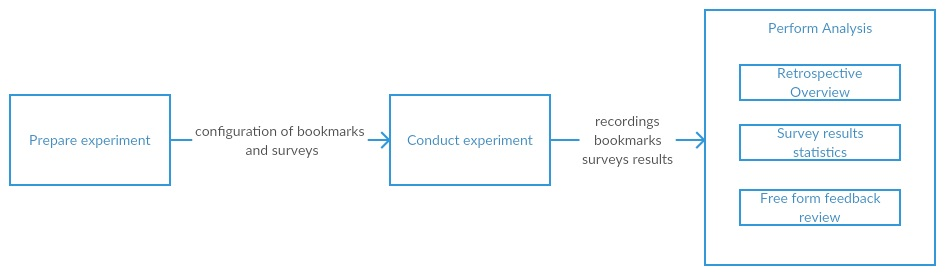
\includegraphics[width=\textwidth]{figures/process.jpg}
\caption{General methodology of MaCon approach evaluation}
\label{fig:process}
 \end{figure}

% During the thesis research there was a test experiment designed and held multiple times to show an example of the user study and how the Analysis Tool works on the data. The detailed description of the experiment and the results are in the Chapter \ref{chapter:evaluation}.


\section{Integrated data collection}\label{section:integrated_data_collection}
In this section we explain the approach for experiment data collection, which includes media files, Bookmarks and Surveys data. This section contains the details of the motivation and usage of this data as well as the general method of collection and description of elements. Media files collection is described in Subsection \ref{subsec:media_files}. Bookmarks, Surveys and Triggers in Subsections \ref{subsec:bookmarks} and \ref{subsec:surveys}.\\

\subsection{Media files collection} \label{subsec:media_files}
As it was mentioned earlier, during the experiments the media data should be collected: screen, audio and video recordings. Collecting the recordings is much better that having the researcher taking notes in the terms of the quantity of useful data, quality of experiment and variety of possible answers retrieved from the data during the analysis. Having all the data gathered during the experiment would be sufficient for the researcher to perform the analysis and evaluation even if the researcher wasn't present at the experiment.\\

Media information is especially important for the evaluation of the engineering process as it captures all the interaction of the team between each other and the software during the experiment and is somehow relevant for the usability evaluation of the modeling technique and the prototyping tool.\\

The audio can capture such important things as discussion of ideas, task division, object specification, state of the system and model, complexities, oral feedback and pretty much anything a team would discuss during the experiment. The video data is more an addition to the audio and screen data and might give a better understanding of users' reaction to the software, process, experiment design etc. Video might be another way of submitting information. The subject might, for example, show some schema drawn on a paper or a whiteboard. The screen recording captures all the interaction of the users with the system and any other software used during the experiment, like chats, browser for searching additional information, etc. The researcher can go to any moment of the experiment and watch or recreate the activities that were happening during that time or the activities that have lead to a certain state of the system. The recording together with the Analysis Tool give a precise, searchable record of subject behavior.\\ 

The media files are collected automatically and the recording start when the workbench is being turned on. This requires no effort from either subject or researcher and saves the experiment from the situation when the participant forgets to turn the recording on or willingly decides to hide the relevant information. Therefore the continuous non-stop recording guarantee that all the relevant information would be present in the experiment results. Of course, the participants need to be warned that there will be recording and that it will start automatically when they launch the software. There is a disadvantage in this decision: it might be uncomfortable for the subjects to have a constant recording of their activity and it might be more complicated to find participants for the study, although the results of the test experiment show that the majority of the participants find it comfortable to have the automatic recording (See Figure \ref{fig:recording_feedback}). The detailed feedback about the integrated data collection is presented in the Chapter \ref{chapter:evaluation} in Section \ref{section:evaluation}.

   \begin{figure}[htb]
 \centering
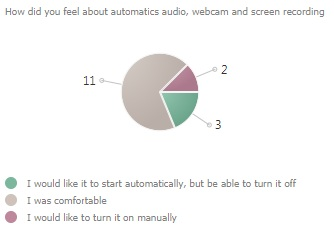
\includegraphics{figures/recording_feedback.jpg}
\caption{Feedback concerning automatic recording}
\label{fig:recording_feedback}
 \end{figure}

\subsection{Bookmarks}\label{subsec:bookmarks}
This part of the data collection is more specific to the activities during the engineering process. The surveys are triggered by the bookmark events, although there can be bookmarks without any survey. One survey is a set of forms that together form a questionnaire window that appears after a certain bookmark event is being fired. It is recommended to design events and surveys in correspondence to the expected activities and milestones the participants are predicted to go through during the experiment. For example, if there is a stage of requirements design in the engineering process, it would make sense to configure a Time Interval bookmark called "Requirements design" to mark the beginning and end of the process and configure a survey which contains questions about requirements creation to be fired when the stage is finished and participant marks the "Requirements design" time interval as "Stop". Therefore the researcher would get the activity bookmarked on the timeline and the feedback about the activity would be collected exactly after it and contain fresh impressions.\\

There are the following types of bookmarks that can be defined in the experiment configuration:

\begin{itemize}
\item Timepoint
\item Time Interval
\item Automatic event
\end{itemize}

\textbf{Timepoint} is a manually triggered event and is represented by a button that calls a survey window as pressed. For example during the test experiment there was an "I've got a problem" button that was offered to be clicked whenever the participant is confused or unsatisfied with the software or the process. It called a window where the subject could select the type of a problem and leave a short feedback about it. \\

\textbf{Time Interval} is a manually triggered event and is a special type of a bookmark designed to capture the continuous process or activity. The Time Intervals are represented by buttons with two states and the participant can switch the state by toggling the button, pressing "Start" and "Stop". The survey window can appear when the activity starts, stops, both or neither.\\

Timepoint and Time Interval can be grouped into event groups for a more comfortable display and added with an icon.\\
 
\textbf{Automatic event} is an event that is triggered by a certain situation inside the workbench. For example in the experiment there was an automatic event that was triggered by the end of the simulation and offered to leave a feedback about the simulation results. There is a big potential of the automatic events in the terms of behavior capturing. The researcher needs to write some code in order to write a trigger class, but it leaves a lot of freedom to submit bookmarks and/or call surveys according to the some situations. Another example of usage of the automatic events would be event that calls a survey every hour. In the configuration file the researcher has to specify the name of the trigger class that has to implement a certain interface and actually write the implementation in the class. For example for triggering a survey after the simulation is done the class SimulationTrigger was written. It sets up a listener and activates a Survey when SimulationEnd event is being published. The details can be found in the  Section \ref{section:dataCollectionIntegration}.\\

UML class diagram of the corresponding objects is presented on the Figure \ref{fig:data_collection_class_diagram}.\\

 \begin{figure}[htb]
 \centering
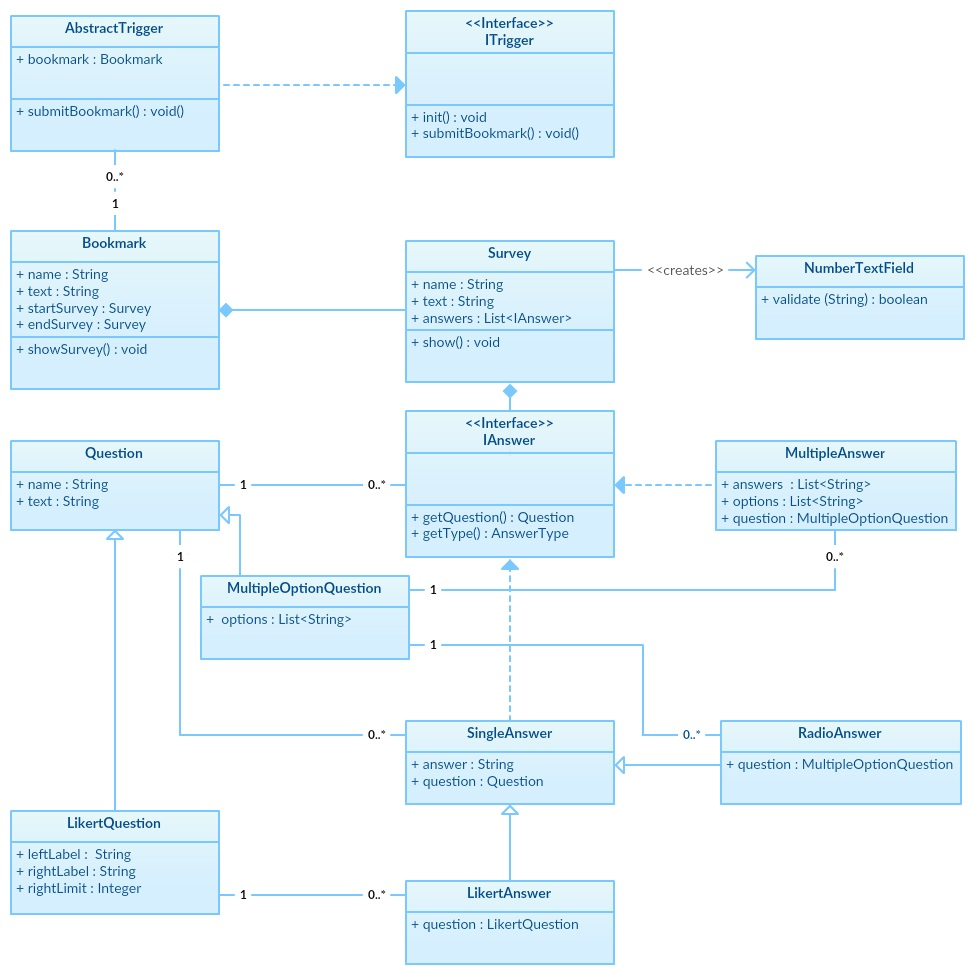
\includegraphics[width=400pt]{figures/data_collection_class_diagram.jpg}
\caption{Class diagram of data collection entities}
\label{fig:data_collection_class_diagram}
 \end{figure}

\subsection{Surveys}\label{subsec:surveys}

The surveys include the following types of the questions:
\begin{itemize}
\item Number
\item Likert scale
\item Multiple choice
\item Single choice
\item Free form feedback
\end{itemize}

Number is a type of a question, where the researcher expects a number as a answer, for example age of the participant. When responding to a Likert questionnaire item, respondents specify their level of agreement or disagreement on a symmetric agree-disagree scale for a series of statements. Thus, the range captures the intensity of their feelings for a given item \cite{wiki:Likert_scale}. Multiple choice is a question where the participant may select none, one or several options among the list of predefined options. Single choice question is a question, where the user has to select one of the predefined options. Free form text feedback question provides a possibility for a subject to leave a custom text as an answer to a question. It's recommended to avoid using Text questions where it's possible to use a predefined question with an "Other" option to submit a custom answer, because they undergo analysis better and require less time and effort from the participants.\\

Free form feedback would be represented as a textarea and a number as an input field with a proper validation. Radiobutton and checkbox are the question representation for questions with predefined answer options. Radiobutton for single answer and checkbox for multiple.  Likert scale is visualized by a slider like on Figure \ref{fig:slider} and offers the user to select the level of agreement between two opposite options. The left and right options as well as the quantity of intermediate steps are configured. It's recommended to keep the position of left and right options the same as well as the quantity of the steps - changes can confuse the user and cause false feedback. \\

You can see an example of a survey on the Figure \ref{fig:survey} and the UML class diagram of the corresponding objects on the Figure \ref{fig:data_collection_class_diagram}.\\
 
 \begin{figure}[htb]
 \centering
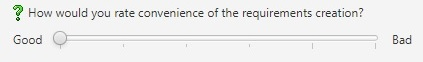
\includegraphics{figures/slider.jpg}
\caption{Slider}
\label{fig:slider}
 \end{figure}
 

 \begin{figure}[htb]
 \centering
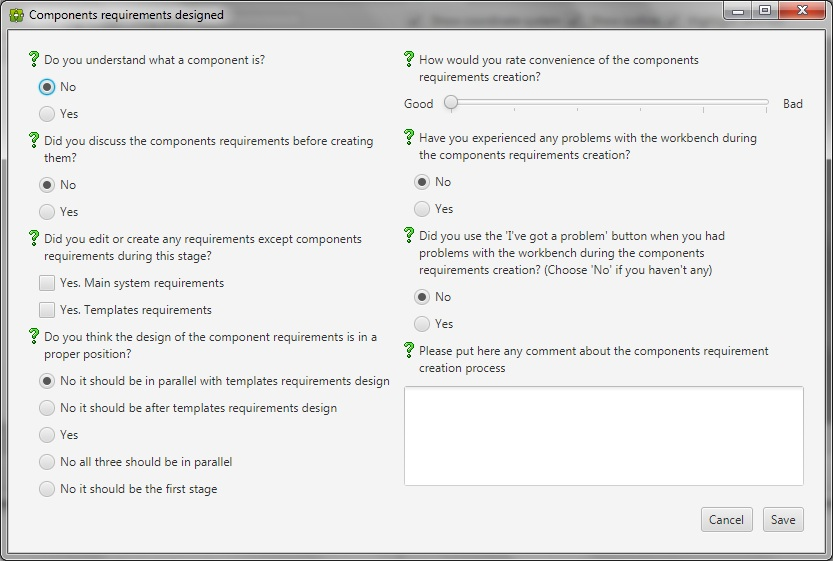
\includegraphics[width=\textwidth]{figures/comp_survey.jpg}
\caption{Survey example}
\label{fig:survey}
 \end{figure}
 
\section{Analysis tool} \label{section:analysis_tool}
The Analysis Tool consists of three parts:overview, statistics and text feedback editor with a navigation between them.

\subsection{Overview}
Overview tab is mainly used during the retrospective project analysis. You can see the Overview window on Figure \ref{fig:overview}. The tab contains the media files players grouped by workstations/sessions with a common timeline. The waveform is convenient for the researcher to navigate to the parts where there  is some sound. The bookmark timeline shows the bookmarks and a click on a bookmark shows the survey answers, if there is a survey attached to the bookmark. You can see this situation on Figure \ref{fig:overview2}. Therefore bookmarks create additional navigation functionality, so the researcher can navigate to certain events and have a detailed look on what was going on before and after the event.\\

 \begin{figure}[htb]
 \centering
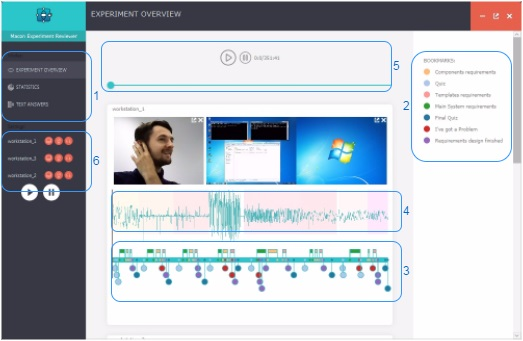
\includegraphics[width=\textwidth]{figures/overview.jpg}
\caption{Overview tab. 1 - navigation pane, 2 - bookmarks pane, 3 - bookmarks timeline, 4 - waveform, 5 - timeline, 6 - settings pane}
\label{fig:overview}
 \end{figure} 
 
  \begin{figure}[htb]
 \centering
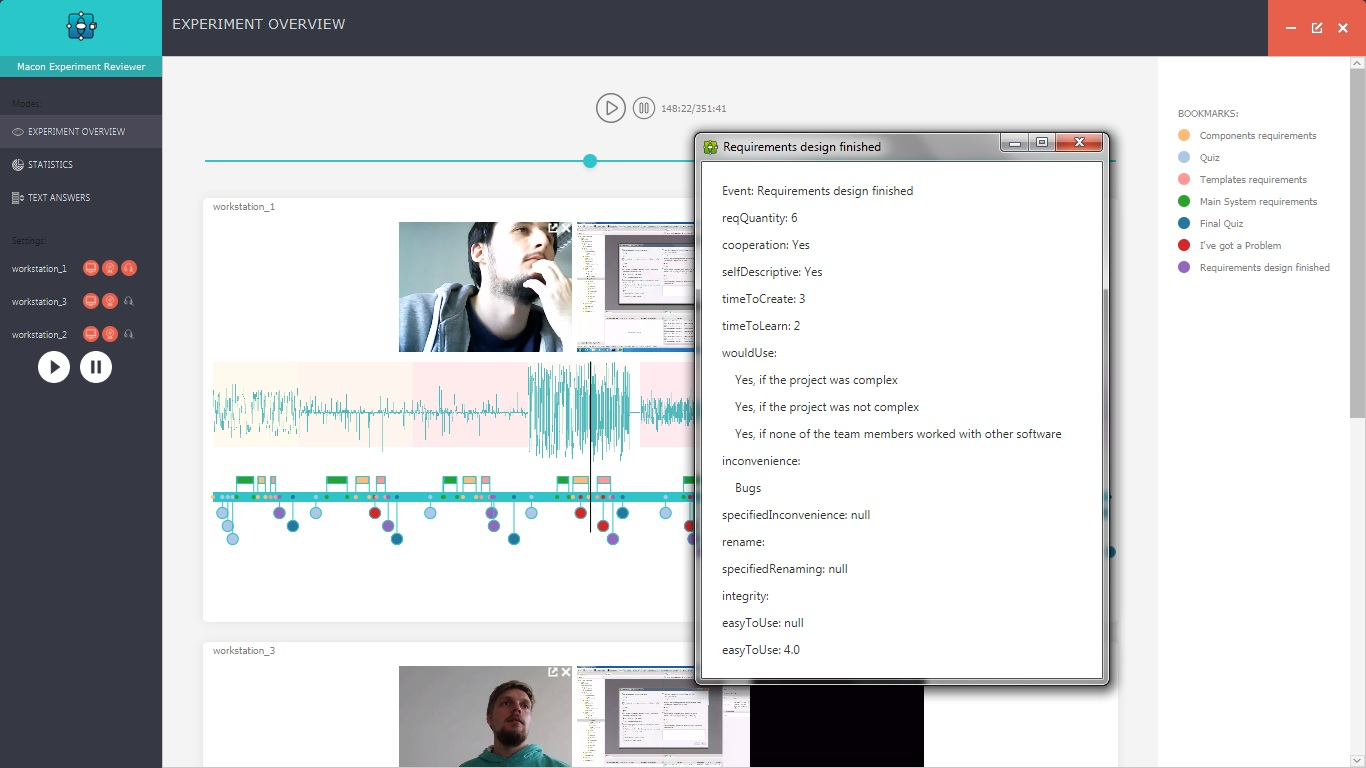
\includegraphics[width=\textwidth]{figures/overview2.jpg}
\caption{Overview tab in the expanded mode with an active bookmark details popup}
\label{fig:overview2}
 \end{figure} 

The left settings pane allows the user to control the player properties: to hide/show screen or webcam players and mute the session. Expanding and collapsing are also possible via proper buttons. The bookmarks panel allows to hide and show events on the bookmark timeline, which simplifies the situation when the researcher is interested in the certain type of events.\\



The example overview tab usage scenario would be as following: The researcher is interested in the context of the system usage that was happening before the participants clicked "I've got a problem" button. The researcher uses the bookmarks panel to filter the bookmarks by type or finds the proper bookmark on the timeline by color. A click navigates him to the proper time and he can see what the subject was doing with the software before the problem occurred as well as what the other teammates were doing. Thus the researcher has a detailed context of the event. He can also use the waveform to navigate to the places where there was sound to find if there was any oral comment about the problem. For example, the researcher might be interested in listening to the discussion the team had before creating some objects. The researcher sees the peaks on the waveform that show there was some sound, most probably conversation, so the researcher navigates to the moments where was some talking to hear the interesting information. \\

You can see the class diagram of objects, that are involved into the Overview functionality of the Analysis Tool on Figure \ref{fig:overview_class_diagram}.\\ 

  \begin{figure}[htb]
 \centering
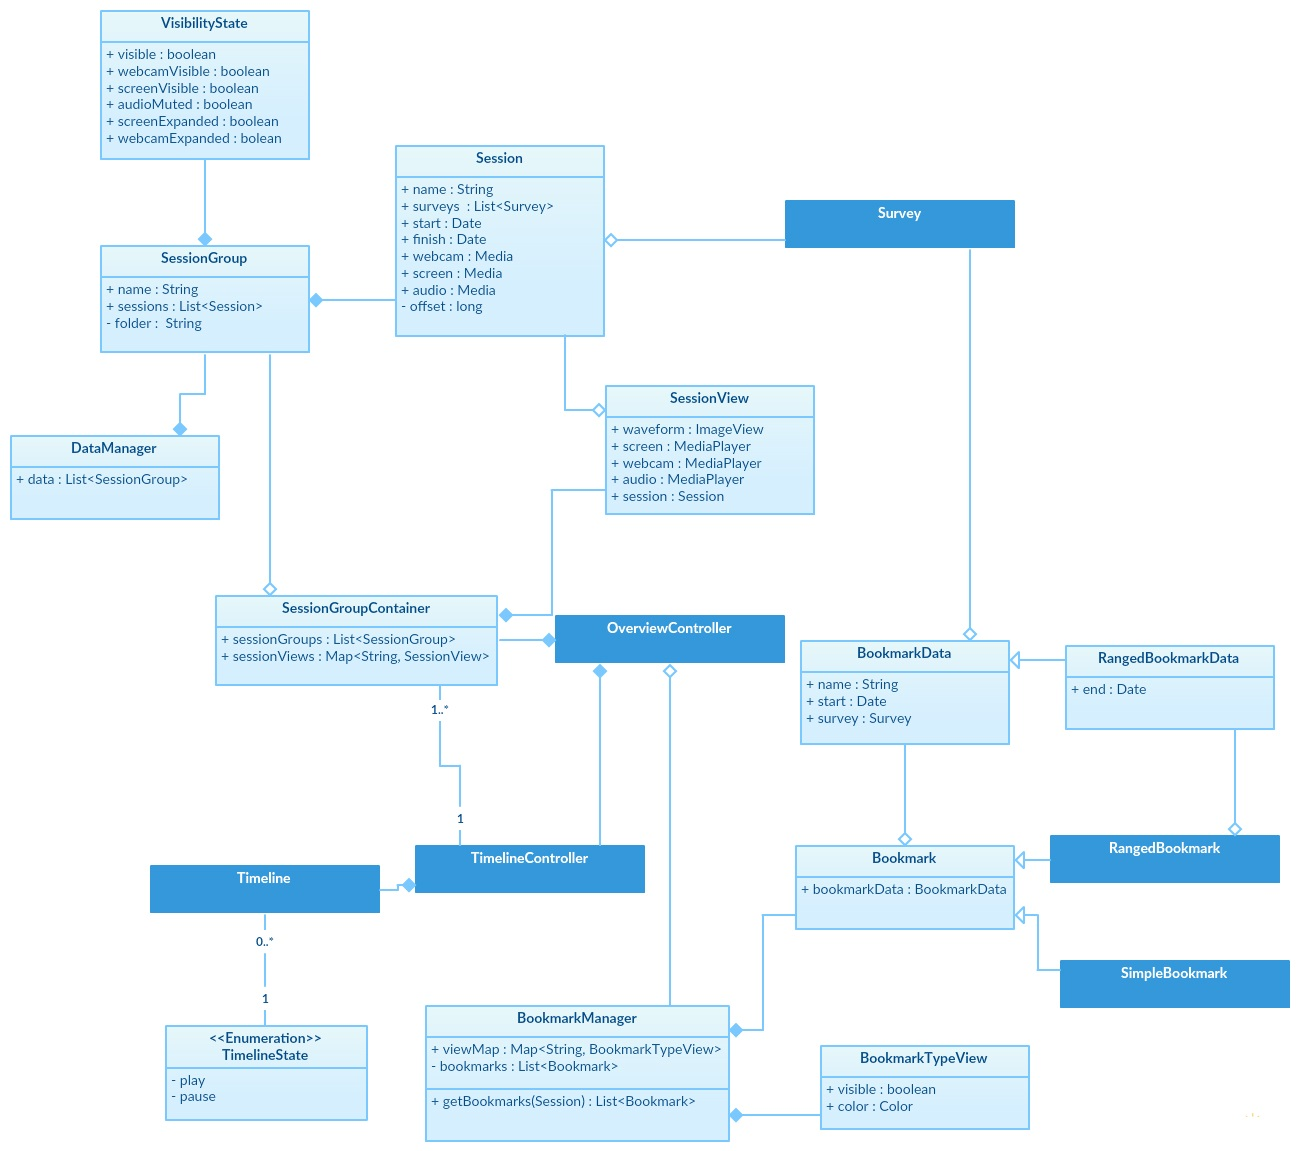
\includegraphics[width=\textwidth]{figures/overview_class_diagram.jpg}
\caption{Overview class diagram}
\label{fig:overview_class_diagram}
 \end{figure} 
 
\subsection{Statistics}

Statistics view gives the researcher the overview on the results of the questionnaires, that participants answered during the experiments. This information can be used for retrospective analysis, evaluation of the modeling technique and overall usability of the software. The results are presented in the form of chart according to the types of the questions.\\

Statistics tab represents a dashboard that shows the results of the surveys (see Figure \ref{fig:statistics}). The left settings pane is for selecting a session for highlighting. If the session is selected all the charts highlight the answer or answer sector for the selected session (see Figure \ref{fig:statistics2}). It would help the researcher to analyze the correlation between the answers. For example there can be a connection between participants' background and experience and how they find the prototyping tool complex to use. Color schema of the carts in a survey window matches the color of the survey form. The user can hide/shop the survey results by toggling the survey visibility in survey pane on the right.\\  

  \begin{figure}[htb]
 \centering
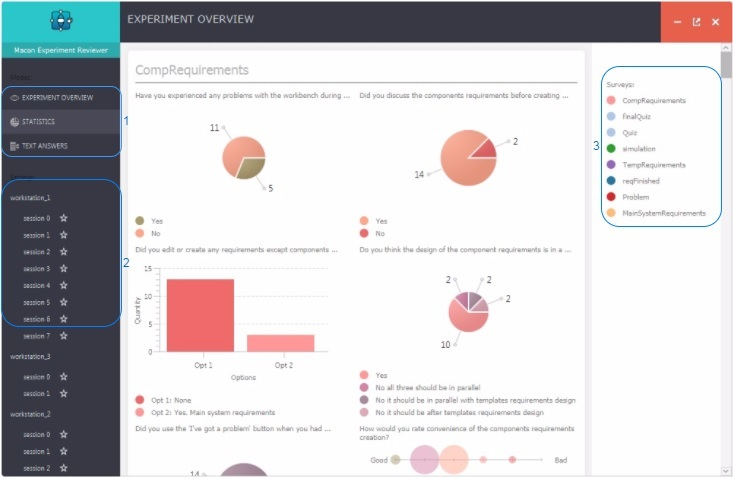
\includegraphics[width=\textwidth]{figures/statistics.jpg}
\caption{Statistics tab. 1 - navigation pane, 2 - settings pane, 3 - surveys pane.}
\label{fig:statistics}
 \end{figure}
 
   \begin{figure}[htb]
 \centering
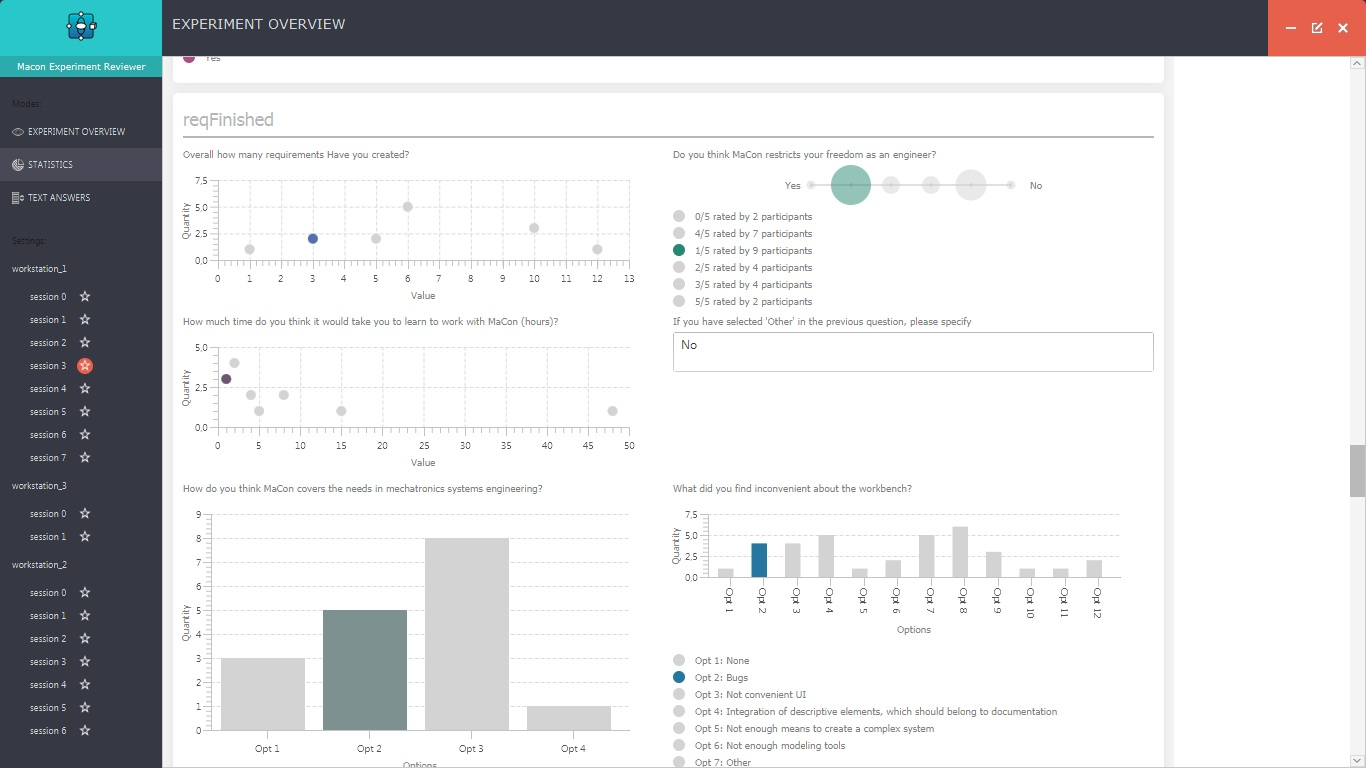
\includegraphics[width=\textwidth]{figures/statistics2.jpg}
\caption{Statistics tab in the expanded mode with session highlighting}
\label{fig:statistics2}
 \end{figure}

Different types of questions are represented by different types of charts (see Figure \ref{fig:visualizations}). The following types of visualizations are used to display survey answers:
\begin{itemize}
\item Pie chart for single choice question
\item Bar chart for multiple choice question
\item Scatter Plot for number questions
\item One dimensional Bubble chart for Likert scale 
\item Text Areas for free feedback
\end{itemize}


\begin{figure}
  \centering
  
  \subfigure[Pie Chart]{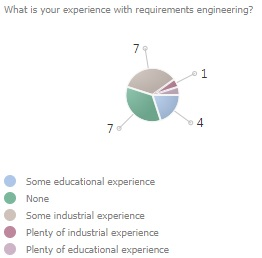
\includegraphics[width=0.36\textwidth]{figures/statistics_pie_chart.jpg}}  
  \subfigure[Bar Chart]{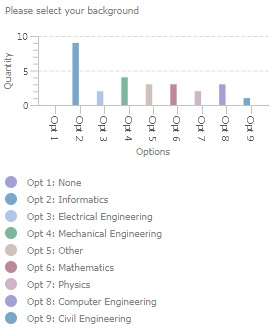
\includegraphics[width=0.36\textwidth]{figures/statistics_bar_chart.jpg}}   
  
   \subfigure[Scatter Plot]{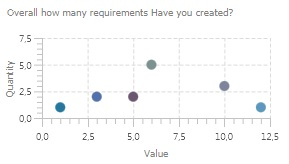
\includegraphics[width=0.36\textwidth]{figures/statistics_scatter_chart.jpg}}      
    \subfigure[Bubble Chart]{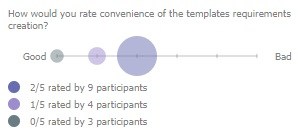
\includegraphics[width=0.36\textwidth]{figures/statistics_likert.jpg}}     
    
        \subfigure[Text Areas]{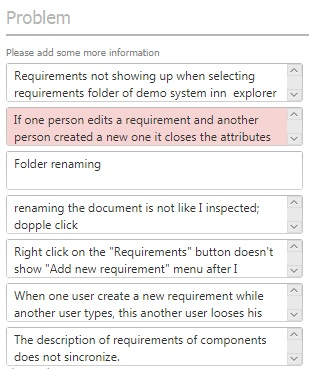
\includegraphics[width=0.36\textwidth]{figures/statistics_text.jpg}} 
    
  \caption{Survey result visualizations}
  \label{fig:visualizations}
\end{figure}


The UML class diagram of the corresponding objects is presented on Figure \ref{fig:statistics_class_diagram}.\\
 
 \begin{figure}[htb]
 \centering
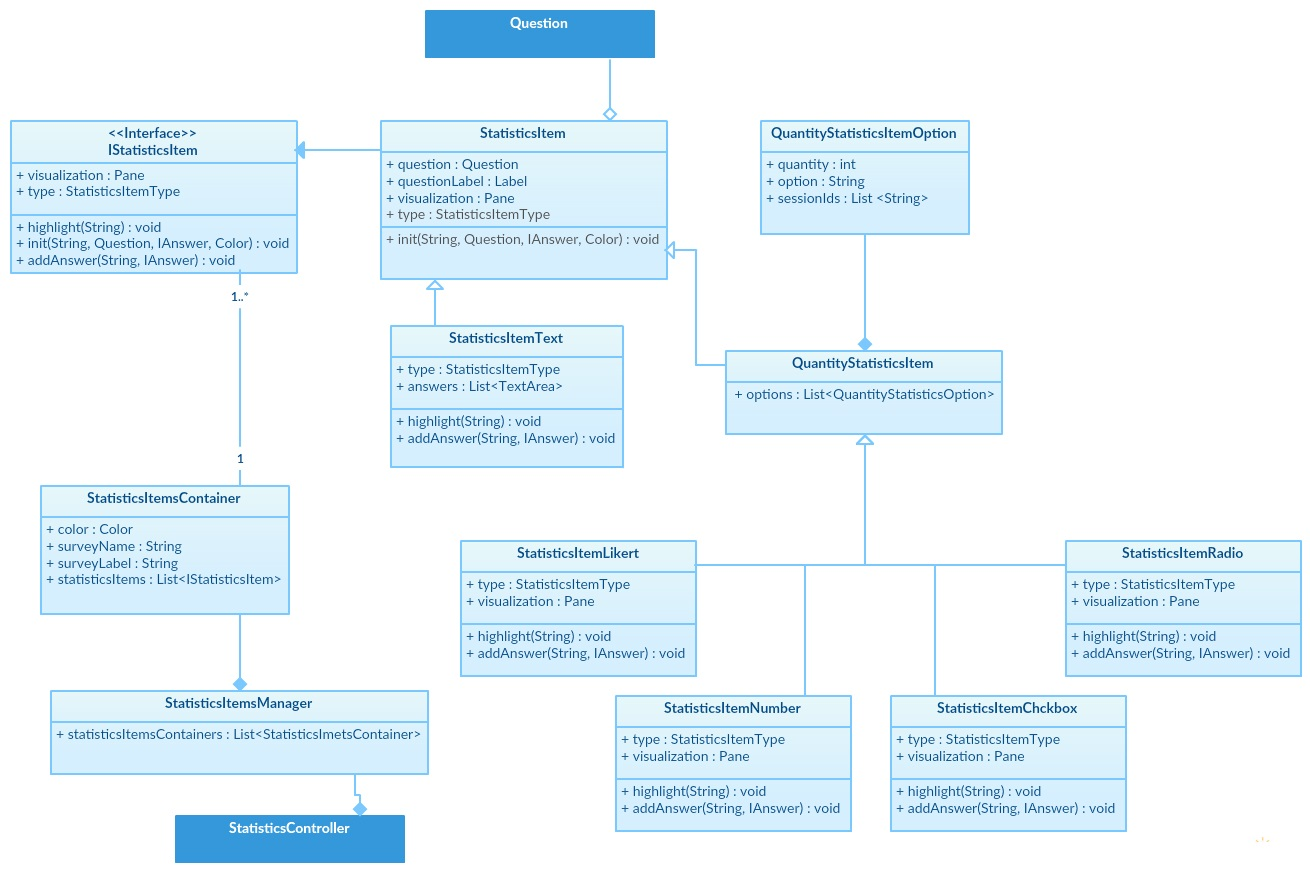
\includegraphics[width=\textwidth]{figures/statistics_class_diagram.jpg}
\caption{Statistics class diagram}
\label{fig:statistics_class_diagram}
 \end{figure}


 
 \subsection{Text Answers}
Text Answers tab is used for the free form feedback analysis. Its almost unavoidable to have free forms for collecting participants' opinions about different aspects of the engineering approach, because it's hard to predict and cover all possible feedback options in predefined options questions. Moreover text feedback might reflect unexpected results about users perception of the approach or software.\\

Plain text is harder to process in terms of extracting overall statistics of participants answers on a question, although usually it might be possible to label the answers and therefore divide the answers into categories. The statistics over the categories might be the scope of interest for the researcher. For example if there is a free form text question about overall impression over the workbench, during analysis the researcher might notice that the answers can be divided into the following categories: positive, neutral, negative. It would be useful to see the ratio of the categories, so the researcher would mark the answers according to the categories and see the visualization of the result. Let's suppose during the analysis, the researcher notices that there is some information repetitively mentioned in the answers, for example some part of the software is inconvenient. It can be mentioned in positive, neutral or negative answers, but the researcher would like to display this knowledge in the visualization. This is why an answer can be labeled as multiple categories.\\

You can see the Text Answers tab on Figure \ref{fig:texts_0}. The left navigation pane provides navigation to other tabs, left settings pane shows the sessions grouped by workstations, so the user could select a session to highlight among the answers. The right pane shows the free form text questions grouped by surveys. The researcher can show/hide the question by toggling the visibility state.\\

 \begin{figure}[htb]
 \centering
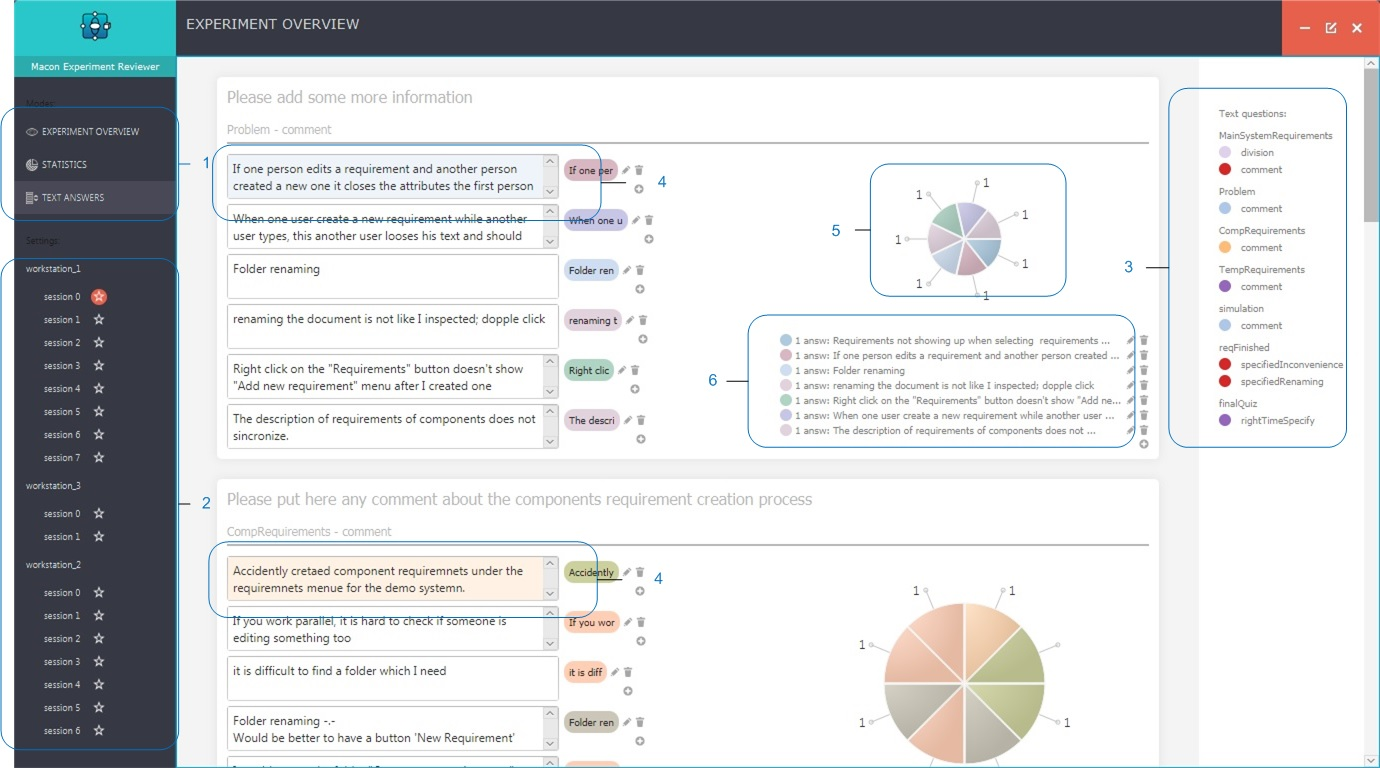
\includegraphics[width=\textwidth]{figures/texts_0.jpg}
\caption{Text answers tab. 1 - navigation pane, 2 - setting pane, 3 - question pane, 4 - highlighted answers, 5 - resulting visualization, 6 - labels.}
\label{fig:texts_0}
 \end{figure}
 
 The initial state of the question view looks like on Figure \ref{fig:texts_1}. As you can see Analysis Tool automatically generates a label for every unique answer. Same answers are automatically grouped with the same label, like answers "\textit{We didn't}" were grouped on the example on the Figure \ref{fig:texts_1}. The researcher is supposed to delete the redundant labels, edit the existing ones and add new labels if necessary. The buttons for doing this are in the labels panel. Near the answers there are buttons to exclude the label from the answer and mark/unmark the answer with labels as well as edit the label. The visualization is updated automatically according to the changes. Editing of the labels allows to change the color and Text. Marking/Unmarking answers offers a list of labels to check. When the new  lable is created it is being assigned with a default unique name and color form the matching color schema. The operations are shown on Figure \ref{fig:texts_3}. \\
 
  \begin{figure}[htb]
 \centering
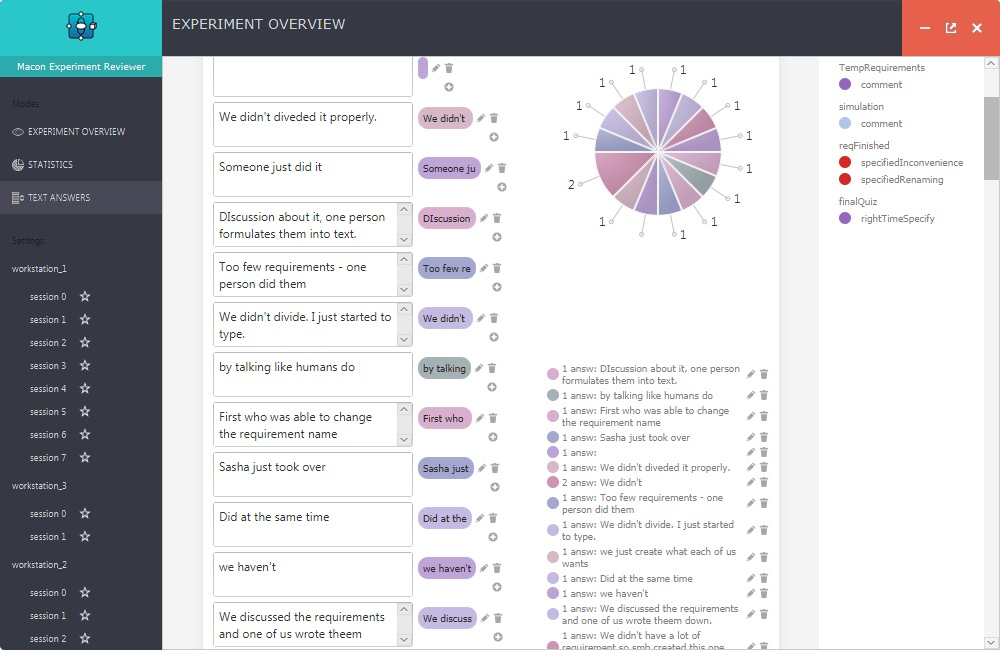
\includegraphics[width=370pt]{figures/texts_1.jpg}
\caption{Initial state of the answers set}
\label{fig:texts_1}
 \end{figure}

 
 \begin{figure}
  \centering 

  \subfigure[Editing of the label]{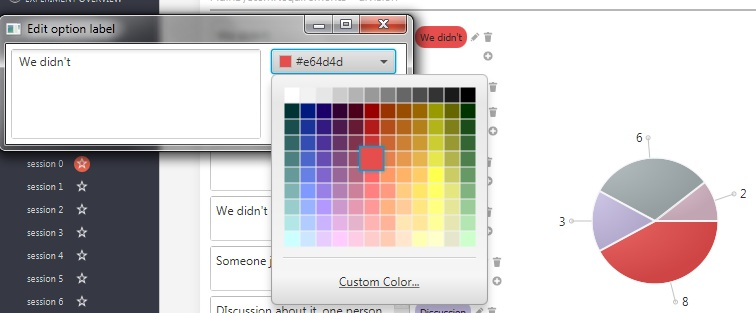
\includegraphics[width=0.3\textwidth]{figures/texts_edit_label.jpg}}      
  \subfigure[Creation of the new label]{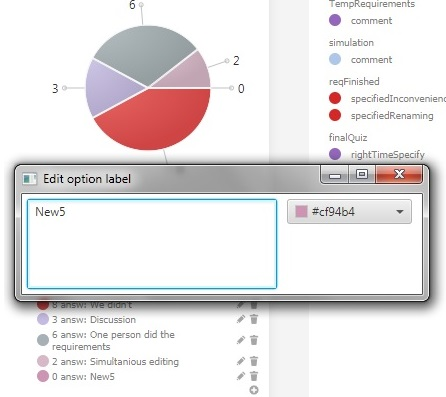
\includegraphics[width=0.23\textwidth]{figures/texts_new_label.jpg}} 
    \subfigure[Marking an answer with labels]{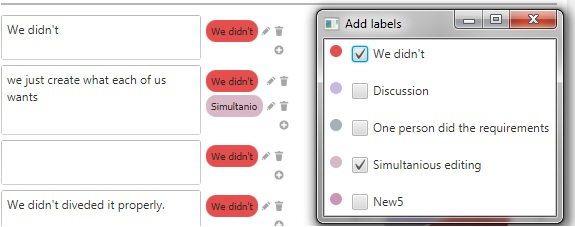
\includegraphics[width=0.3\textwidth]{figures/texts_add_label.jpg}}  
    
  \caption{Operations in Text Answers tab}
  \label{fig:texts_3}
\end{figure}
 
 You can see how the answers set looks after the researcher has worked with the tool on the Figure \ref{fig:texts_2}. As you can see, the labels were edited, and the answers were marked with the proper labels, so the visualization looks meaningful. \\
 
   \begin{figure}[htb]
 \centering
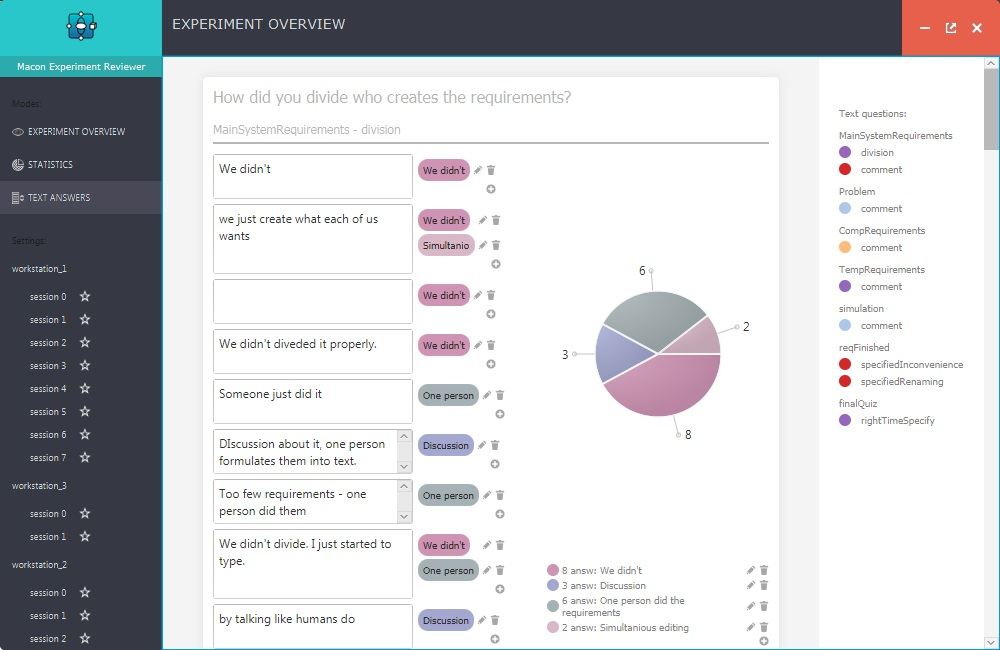
\includegraphics[width=370pt]{figures/texts_2.jpg}
\caption{Answer set after editing}
\label{fig:texts_2}
 \end{figure} 


The UML class diagram of the corresponding objects is presented on Figure \ref{fig:texts_class_diagram}.\\
 
    \begin{figure}[htb]
 \centering
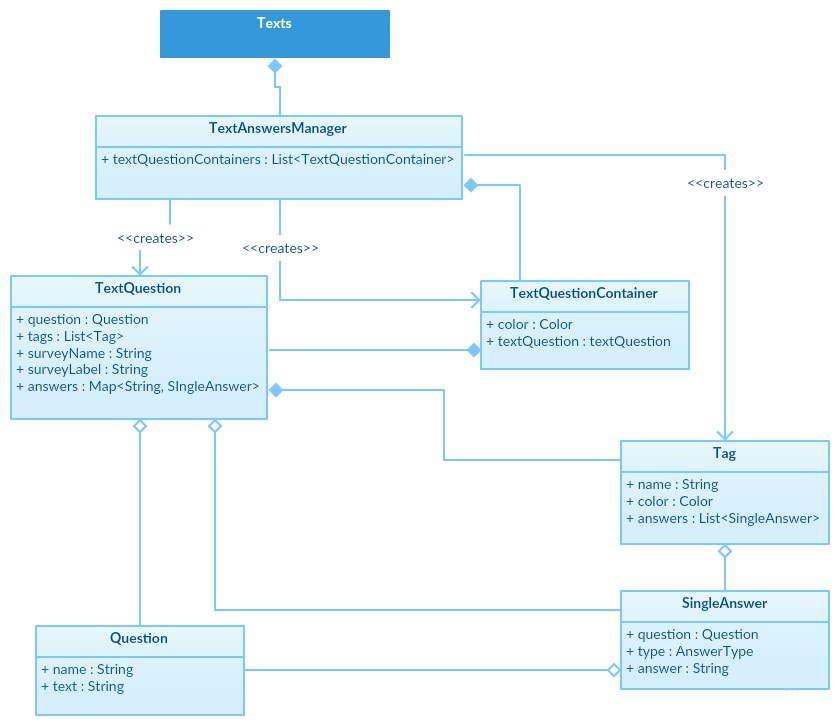
\includegraphics[width=290pt]{figures/texts_class_diagram.jpg}
\caption{Text answers class diagram}
\label{fig:texts_class_diagram}
 \end{figure}


